\documentclass{article}
\title{Blanchard Ch.18}
\author{Dawei Wang}
\date{\today}
\usepackage{ctex}
\usepackage{amsmath}
\usepackage{amssymb}
\usepackage{graphicx} %插入图片的宏包
\usepackage{float} %设置图片浮动位置的宏包
\usepackage{subfigure} %插入多图时用子图显示的宏包
\begin{document}
	\maketitle
	
\section{开放经济中的IS曲线}
当经济处于开放状态,一些国内需求由外国产品满足,而对国内产品的部分需求来自外国消费者。

\subsection{对国内产品的需求}

在一个开放经济中,对国内产品的需求(demand for domestic goods):

\[
Z=C+I+G-IM/\epsilon+X
\]

前三个项目分别是消费C、投资I和政府支出G,构成了对产品的国内需求(domestic demand for goods),包括国内产品和外国产品。如果经济是封闭的,C+I+G也就是对国内产品的需求,开放情形下需要做两处调整:

1. 必须减掉进口,它意味着部分国内需求落到了外国产品而不是国内产品上,$ \epsilon $代表实际汇率,等价地,$ IM/\epsilon $代表用国内产品表示的进口价值;

2. 必须加上出口,它意味着对国内产品的部分需求来自海外。

\subsection{C、I和G的决定因素}

国内需求:

\[
C+I+G=C(Y-T)+I(Y,r)+G
\]

\subsection{进口的决定因素}

进口是指部分国内需求落到外国产品上。进口取决于国内收入:国内收入越高,对国内产品和外国产品的需求都会越高。进口还显然取决于实际汇率,即用外国产品表示的国内产品价格。国内产品相对于外国产品元昂贵,等价地,外国产品相对于国内产品越便宜,那么对外国产品的国内需求也就越大。所以,一个较高的实际汇率会带来较高的进口:

\[
IM=IM(Y,\epsilon)
\]

\subsection{出口的决定因素}

出口是指外国的部分需求落到国内产品上。它取决于外国收入:更高的外国收入意味着对所有产品的更高的需求水平。出口也取决于实际汇率:用外国产品表示的国内产品的价格,对国内产品的外国需求也就越低。实际汇率越高,出口越低。

用$ Y^* $表示外国收入,我们可以将出口写成:

\[
X=X(Y^*,\epsilon)
\]

\subsection{把所有因素加总起来}

\begin{figure}[H] %H为当前位置,!htb为忽略美学标准,htbp为浮动图形
	\centering %图片居中
	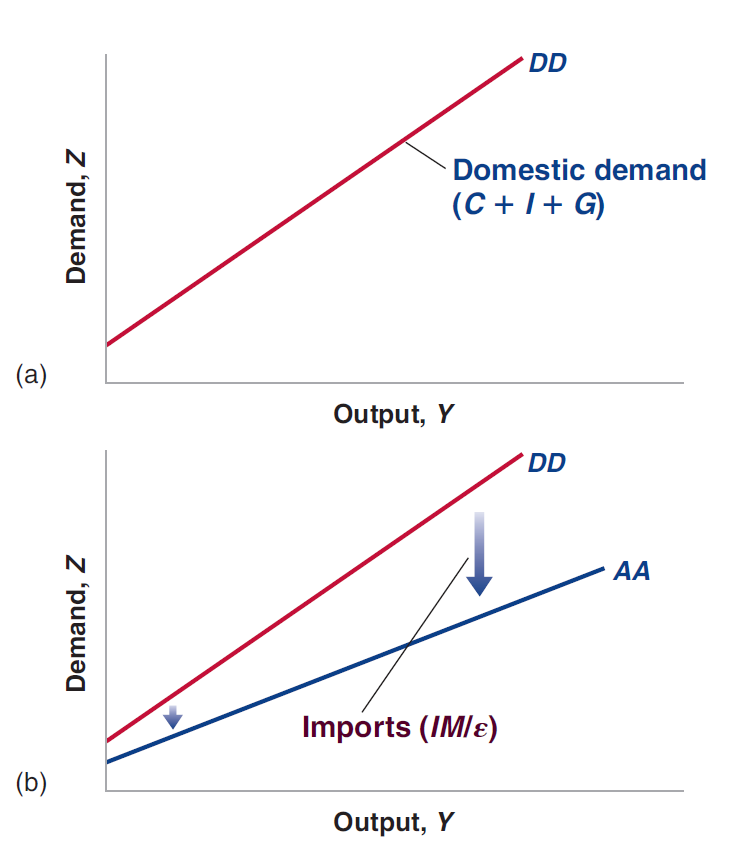
\includegraphics[width=1\textwidth]{18_1} %插入图片,[]中设置图片大小,{}中是图片文件名
	\caption{} %最终文档中希望显示的图片标题
	\label{Fig.main2} %用于文内引用的标签
\end{figure}

\begin{figure}[H] %H为当前位置,!htb为忽略美学标准,htbp为浮动图形
	\centering %图片居中
	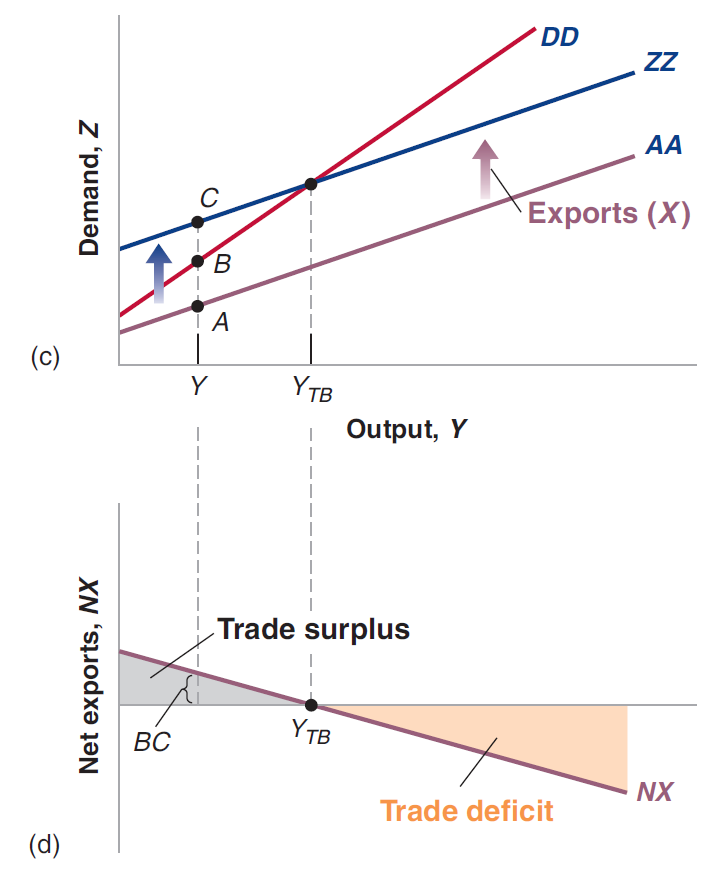
\includegraphics[width=1\textwidth]{18_2} %插入图片,[]中设置图片大小,{}中是图片文件名
	\caption{The Demand for Domestic
		Goods and Net Exports} %最终文档中希望显示的图片标题
	\label{Fig.main3} %用于文内引用的标签
\end{figure}

DD线和AA线之间的距离等于进口的价值$ IM/\epsilon $。由于进口数量伴随着收入的提高而增加,那么这两条线之间的距离也随着收入的增加而变大。

AA线的特点:

AA线比DD线更平坦:随着收入增加,一些新增的国内需求落到了外国产品上而不是国内产品上。随着收入的增加,对国内产品的国内需求的增加幅度要小于总需求的增加。

只要一些新增的需求落到国内产品上,AA线就有一个正的斜率,收入的增加导致对国内产品需求的部分增加。

加上出口得到ZZ线,ZZ线在AA线以上。ZZ线代表了对国内产品的需求。ZZ线和AA线间的距离等于出口,由于出口并不依赖于国内收入,ZZ线和AA线之间的距离是一定的,两条线平行。

净出口于贸易余额是同义的,正的净出口对应着贸易盈余,负的净出口对应贸易赤字。

$ NX=X-IM/\epsilon $表示净出口:随着产出增加,进口增加,但出口并不受此影响,从而净出口下降。用$ Y_{TB} $表示当进口于出口价值相等时的产出水平,此时净出口等于0。产出水平在$ Y_{TB} $以上将导致更高的进口和贸易赤字。产出水平低于$ Y_{TB} $将导致较低的进口和贸易余额。

\section{均衡产出和贸易余额}

在国内产出等于国内外对国内产品的需求时,产品市场达到均衡点:

\[
Y=Z
\]

即:

\[
Y=C(Y-T)+I(Y,r)+G-IM(Y,\epsilon)/\epsilon+X(Y^*,\epsilon)
\]

\begin{figure}[H] %H为当前位置,!htb为忽略美学标准,htbp为浮动图形
	\centering %图片居中
	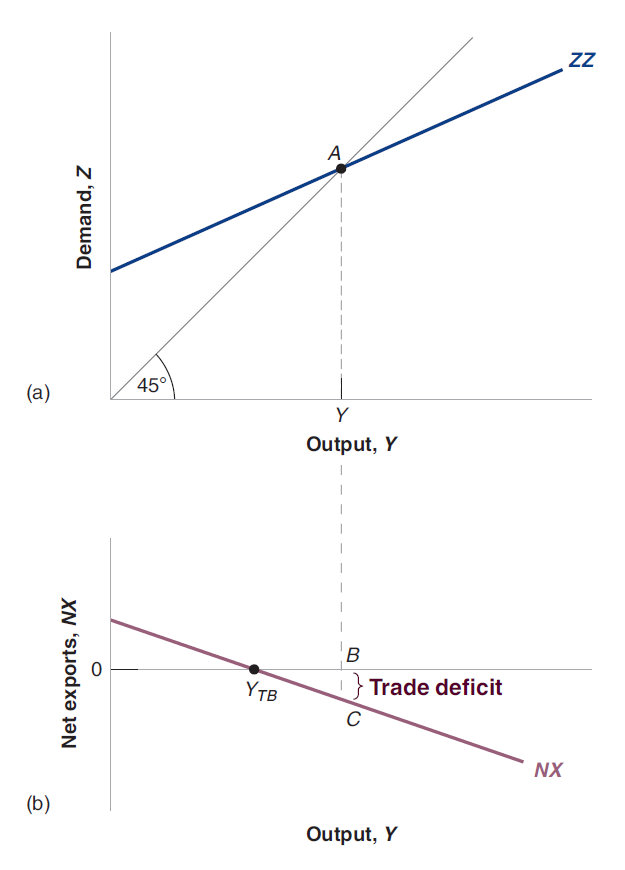
\includegraphics[width=1\textwidth]{18_3} %插入图片,[]中设置图片大小,{}中是图片文件名
	\caption{Equilibrium Output and
		Net Exports} %最终文档中希望显示的图片标题
	\label{Fig.main4} %用于文内引用的标签
\end{figure}

在国内产出等于对国内产品的需求时,产品市场是均衡的。在产出的均衡水平上,贸易余额可能会表现出赤字或者盈余。

产出的均衡水平由条件$ Y=Z $决定。贸易平衡时的产出水平由条件$ X=IM/\epsilon $决定。

\section{国内外需求的增加}

\subsection{国内需求的增加}

假设经济处于衰退之中,政府决定增加政府支出以增加国内需求和产出。假定贸易初始是平衡的。

\begin{figure}[H] %H为当前位置,!htb为忽略美学标准,htbp为浮动图形
	\centering %图片居中
	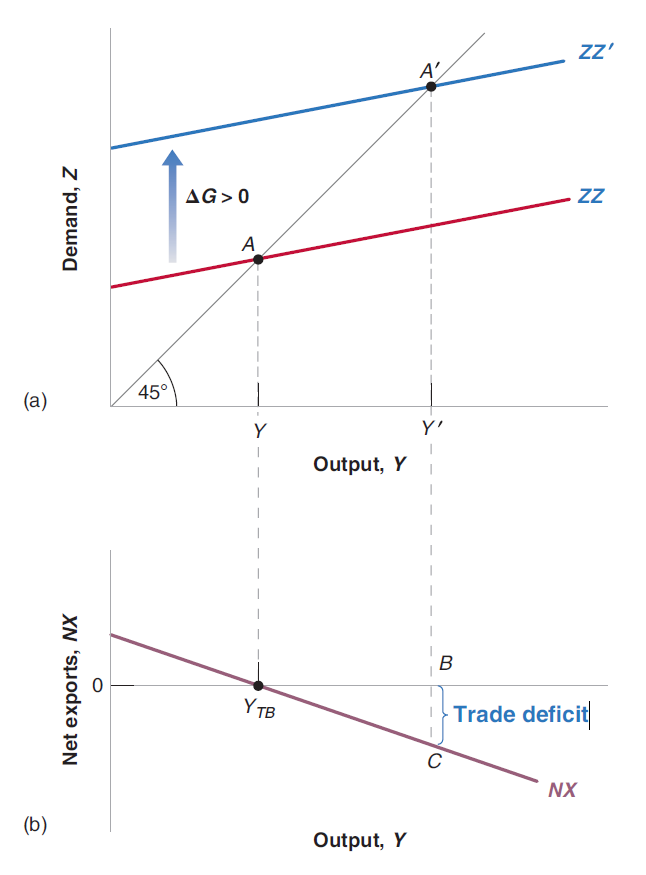
\includegraphics[width=1\textwidth]{18_4} %插入图片,[]中设置图片大小,{}中是图片文件名
	\caption{The Effects of an Increase
		in Government Spending} %最终文档中希望显示的图片标题
	\label{Fig.main5} %用于文内引用的标签
\end{figure}

政府支出增加$ \Delta G $,需求曲线向上移动$ \Delta G $,产出的增加要比政府支出的增加大,这是因为存在乘数效应。

与封闭经济的不同之处:

现在存在一个对贸易余额的效应。产出增加导致进口增加,出口并未改变,贸易赤字增加。

政府支出不仅导致贸易赤字,而且政府支出的产出效应要比封闭经济条件下小。

以上两种效应的原因相同:一些国内需求落在了外国产品上,而不是国内产品上。

在一个开放经济中,国内需求的增加要比在一个封闭经济中对产出的效应要小,并对贸易余额有一个负向作用。事实上,经济越开放,产出效应越小,对贸易余额的负向效应越大。

\subsection{国外需求的增加}

现在假设外国的产出增加了,即$ Y^* $增加。

假定贸易是平衡的。

\begin{figure}[H] %H为当前位置,!htb为忽略美学标准,htbp为浮动图形
	\centering %图片居中
	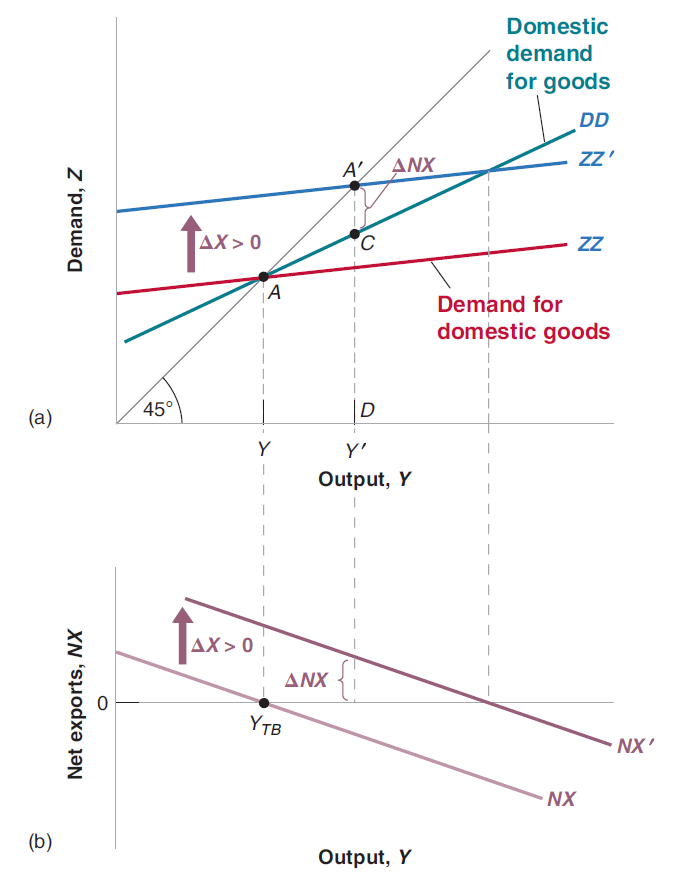
\includegraphics[width=1\textwidth]{18_6} %插入图片,[]中设置图片大小,{}中是图片文件名
	\caption{The Effects of an Increase
		in Foreign Demand} %最终文档中希望显示的图片标题
	\label{Fig.main6} %用于文内引用的标签
\end{figure}

把代表对产品的国内需求(C+I+G)的直线当作收入的函数,称之为DD曲线。DD曲线比ZZ曲线要陡峭。ZZ和DD之间的差额等于净出口因此如果A点的贸易是平衡的,则ZZ和DD在A点相交。

在一个给定的产出水平下,出口的增加将导致国内产品的需求增加$ \Delta X $,从而代表国内产品的需求向上移动$ \Delta X $。

在一个给定的产出水平下,净出口增加$ \Delta X $。表示净出口是产出的函数的直线也向上移动$ \Delta X $。

外国产出的增加将导致国内产出的增加。更高的国外产出导致更高的国内产品出口,这将在乘数效应下增加国内产出和对产品的国内需求。

贸易余额得到改善。当外国需求增加时,贸易余额肯定会得到改善。当外国需求增加时,对国内产品的需求将上移,但是对产品的国内需求是产出的函数的DD线不会移动。在这个新的均衡产出水平$ Y' $下,国内需求由距离DC给定,对国内产品的需求由$ DA' $给定。因此净出口就是距离$ CA' $,因为DD必然处在$ ZZ' $下,$ CA' $也必然为正值。因此当进口增加时,该增加比没有完全抵消出口的增加,贸易余额还是得到改善。

\subsection{重新审视财政政策}

国内需求的增加将导致国内产出的增加,但也会导致贸易余额的恶化。

外国需求的增加导致国内产出的增加和贸易余额的改善。

政府不喜欢贸易赤字,主要的原因是持续出现贸易赤字的国家会累积对世界上其他国家的债务,因而必须向其他国家支付稳定增长的利息。因此,每个国家都偏好外国需求的增加而不是国内需求的提高。

这意味着一国需求的冲击会影响所有其他国家。国家间的贸易联系越紧密,相互影响越深刻,且更多的国家将同步变动。

经济衰退时期若所有国家都担心自己的财政政策的外溢效应而不推迟采用财政政策,经济衰退可能持续很长时间。

\subsection{贬值、贸易余额和产出}

假设政府采取措施导致本币贬值,即名义汇率下降。

\[
\epsilon=\frac{EP}{P^*}
\]

在短期,假设两个价格水平$ P $和$ P^* $是给定的。

\subsection{贬值和贸易余额:马歇尔——勒纳条件}

净出口定义:

\[
NX=X-IM/\epsilon
\]

即:

\[
NX=X(Y^*,\epsilon)-IM(Y,\epsilon)/\epsilon
\]

实际贬值的效应:

1. 出口提高。实际贬值将使本国产品相对于外国产品便宜。这导致对本国产品的外国需求增加,即出口增加。

2. 出口IM下降。实际贬值将使外国产品在本国变得相对昂贵,这导致国内需求向国内产品转换,从而导致进口数量下降。

3. 用国内产品表示的外国产品的相对价格$ 1/\epsilon $增加。这将增加进口的费用$ IM/\epsilon $。进口同样的数量现在将花费更多的购买成本。

为了贬值能够使贸易余额得到改善,出口必须提高足够多,进口也必须降低足够多以抵消进口价格的上升。实际贬值带来净出口提高的条件就是马歇尔——勒纳条件(Marshall-Lerner condition)。

假定实际贬值,即$ \epsilon $下降将导致净出口增加,即NX增加(马歇尔——勒纳条件成立)。

\subsection{贬值的影响}

净出口会改变国内产出,这将进一步影响净出口。

与外国产出的提高相类似,在任何产出水平下,贬值将导致净出口的提高(假定马歇尔——勒纳条件成立)。需求关系ZZ和净出口关系NX都向上移动。均衡点从A点移动到$ A' $点,产出也从Y提高到$ Y' $。贸易余额得到改善:由产出提高引起的进口提高小于由贬值带来的对贸易余额的改善。

总结:贬值使国外和国内的需求都向国内产品转移。这种需求的转换反过来导致国内产出的提高和贸易余额的改善。

尽管贬值和国外产出的提高对国内产出与贸易余额有同样的影响,但这两种效应之间有一个不起眼但很重要的区别。贬值是通过使外国产品相对更贵来起作用的。这就意味着在收入水平给定的情况下,人们的生活水平恶化了。

\subsection{将汇率和财政政策结合起来}

\begin{figure}[H] %H为当前位置,!htb为忽略美学标准,htbp为浮动图形
	\centering %图片居中
	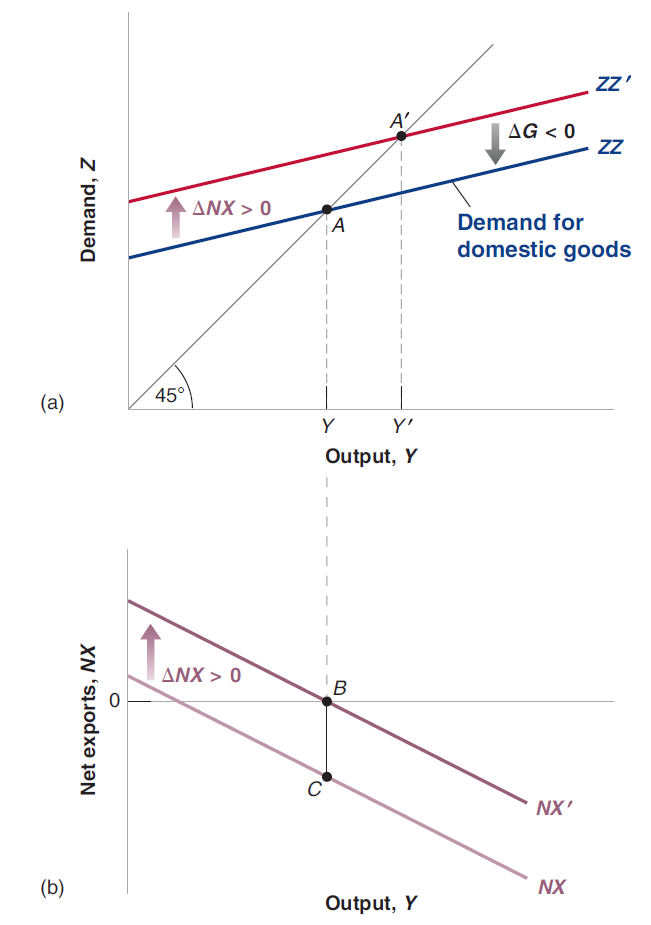
\includegraphics[width=1\textwidth]{18_7} %插入图片,[]中设置图片大小,{}中是图片文件名
	\caption{Reducing the Trade Deficit
		without Changing Output} %最终文档中希望显示的图片标题
	\label{Fig.main7} %用于文内引用的标签
\end{figure}

假设经济处于自然产出水平,但经济大规模的贸易赤字。为了防止经济过热,政府希望在产出不变的条件下减少贸易赤字。政府应采用贬值和适当的财政紧缩政策。

政府应:

1. 必须在初始的产出水平上实现充分的贬值以消除贸易赤字。贬值必须要能使净出口关系中NX转移到$ NX' $。

2. 为了避免产出提高,政府必须减少政府支出以使$ ZZ' $移回ZZ的位置。这种贬值和财政紧缩的结合使产出水平保持不变,同时贸易余额得到改善。

\hspace*{\fill}

一个一般性结论:

如果想达到两个目标,就最好有两个工具。

\begin{figure}[H] %H为当前位置,!htb为忽略美学标准,htbp为浮动图形
	\centering %图片居中
	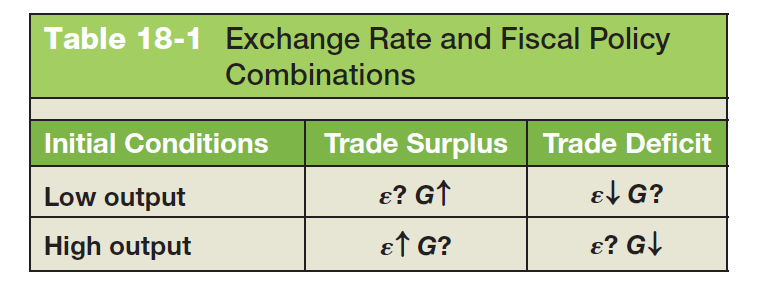
\includegraphics[width=1\textwidth]{18_8} %插入图片,[]中设置图片大小,{}中是图片文件名
	\caption{} %最终文档中希望显示的图片标题
	\label{Fig.main8} %用于文内引用的标签
\end{figure}

\section{考察动态变化:J曲线}

贬值将导致出口增加、进口下降,但这种变动并非一蹴而就。

在贬值发生后几个月,贬值的影响更多地反映在价格上而非数量上。进口产品价格上升,而向外国出口的产品价格下降。但进口和出口数量上的调整可能是缓慢的。因此,贬值在初始阶段将导致贸易余额出现恶化;$\epsilon$下降,但初始阶段的X和IM都没调整,这就导致了净出口(X-IM/$\epsilon$)的下降。

随着时间推进,进口和出口相对价格变化的效应越加强烈。本国产品的低价格将导致消费者和企业降低对外国产品的需求,进口下降。本国产品在海外价格下降,出口增加。如果马歇尔-勒纳条件始终成立,那么出口和进口量的反应最终要比负向作用更为强烈,贬值的最终影响是贸易余额的改善。

\begin{figure}[H] %H为当前位置,!htb为忽略美学标准,htbp为浮动图形
	\centering %图片居中
	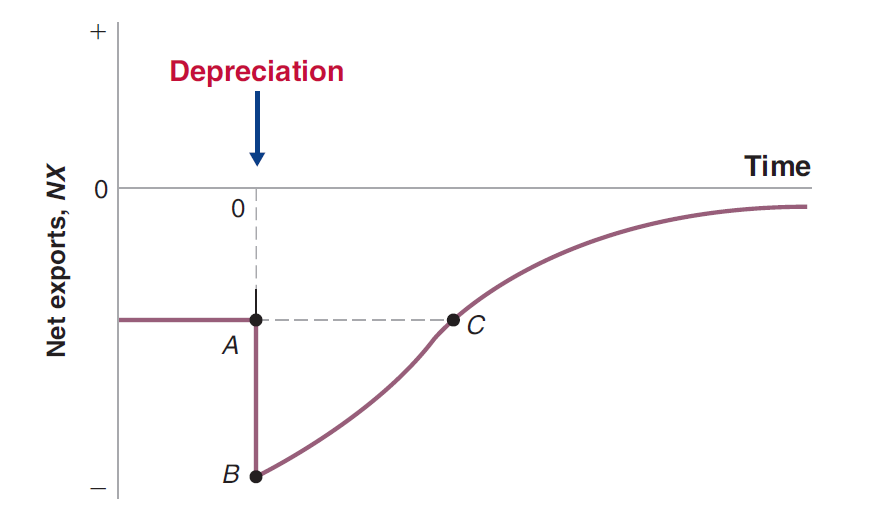
\includegraphics[width=1\textwidth]{18_9} %插入图片,[]中设置图片大小,{}中是图片文件名
	\caption{The J-Curve} %最终文档中希望显示的图片标题
	\label{Fig.main9} %用于文内引用的标签
\end{figure}

1. 实际汇率的变动反应在净出口的平行变动上。升值对应着贸易赤字的急剧增加,而随后的贬值则伴随着贸易余额的大幅下降。

2. 贸易余额对实际汇率变动的反应有着相当时长的滞后。这种滞后不仅仅存在于贬值对贸易余额的影响上,也体现在贬值对产出的影响上。如果贬值最初降低了净出口,那么在开始的时候也会对产出造成负面影响。因此如果政府依赖于贬值来改善贸易余额以及扩大国内产出,那么在一段时间内,其影响将是“适得其反”的。

\section{储蓄、投资和贸易余额}

均衡条件:

\[
Y=C+I+G-IM/\epsilon+X
\]

在开放经济中,国内居民收入等于产出Y,加上从国外得到的净收入NI,再加上收到的净转移支付。将这些转移支付记为NT:

\[
(Y+NI+NT-T)-C=I+(G-T)+(NX+NI+NT)
\]

左边括号内的项目等于可支配收入,所以左侧等于可支配收入减去消费,也就是储蓄S。

净出口、从国外获得的净收入以及净转移支付之和等于经常账户CA。

\[
S=I+(G-T)+CA
\]

即:

\[
CA=S+(T-G)-I
\]

经常账户余额等于储蓄(个人储蓄与公共储蓄之和)减去投资。经常账户盈余意味着该国储蓄多余投资,经常账户赤字意味着该国储蓄少于投资。

经常账户余额意味着该国向世界其他国家净贷出,经常账户赤字意味着该国向世界上其他国家净借入。因此假设一个国家投资超过储蓄,则$ S+(T-G)-I $是负的。该国就必须从世界上其他国家借入这一差额,从而必然存在贸易赤字。反之必须向其他国家贷出这一差额。

\hspace*{\fill}

投资的增加必然反映出私人储蓄的增加或公共储蓄的积累,或贸易余额的恶化;

政府预算余额的恶化必然表现为私人储蓄增加,或投资下降,或经常账户余额恶化;

如果一个国家的储蓄率(私人储蓄+公共储蓄)较高,那么该国就必然有一个较高的投资率或大量的经常账户盈余。

上式不能说明政府预算赤字是否将导致经常账户赤字、私人储蓄增加或投资减少。

	
	
\end{document}